
\section{}
\begin{frame}[allowframebreaks]{Predictive brain - Transformers as predictors for Klaman filter}
    Since different segment composition of language form different meanings, LSTMs (and consequently RNNs) can not catch local dependencies. A multi attention predictor is needed. The transformers \cite{vaswani-2017-attention-is-all-you-need}
    
    Its application here is to replace the constant speed predictor
    
    
    
    \begin{itemize}
        \item At lowest level in each cell, it holds an AP wave represented by FMM
        \item Training
        \begin{itemize}
            \item Deep learning as an autocorrelation to find periods
        \end{itemize}
        \item Sliding windows to train the transformer
        \item Period sampling with auto corrlation for training and validating the transformer
        \item Noise as uncertainty in transformer
    
    \end{itemize}
    \begin{figure}[H]
        \centering
        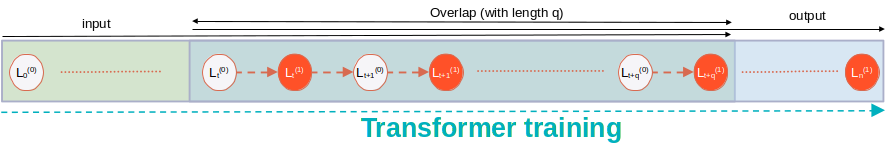
\includegraphics[width=0.9\textwidth]{building_predictive_model/internal_language_building/transformer/transformer.png}
    \end{figure}
    
    \section{Previous}
    Transition matrix
\end{frame}
    \subsection{}
    \begin{frame}[allowframebreaks]{Gaussian Transformer: What It Does}
    \small
    
    The model receives a past time-series window and predicts a future window with uncertainty.
    
    \vspace{0.3cm}
    
    \[
        f_{\theta}:
        \mathbb{R}^{T_{\mathrm{in}} \times F_{\mathrm{in}}}
        \rightarrow
        \mathbb{R}^{T_{\mathrm{out}} \times 2F_{\mathrm{out}}}
    \]
    
    \vspace{0.2cm}
    
    For each future time step and feature, it predicts two values:
    
    \[
        \hat{Y}_{\mathrm{params}}
        =
        [
        \mu,
        \log \sigma^2
        ]
    \]
    
    \vspace{0.2cm}
    
    \[
        y_{b,t,j}
        \sim
        \mathcal{N}
        (
        \mu_{b,t,j},
        \sigma^2_{b,t,j}
        )
    \]
    
    \vspace{0.2cm}
    
    \begin{itemize}
        \item \(\mu\): expected future value
        \item \(\sigma^2 = \exp(\log \sigma^2)\): predictive uncertainty
    \end{itemize}
\end{frame}





    \begin{frame}[allowframebreaks]{Training Loss and Uncertainty Meaning}
    \small
    
    The model is trained with Gaussian negative log-likelihood:
    
    \[
        \mathcal{L}
        =
        \frac{1}{BT_{\mathrm{out}}}
        \sum_{b=1}^{B}
        \sum_{t=1}^{T_{\mathrm{out}}}
        \sum_{j=1}^{F_{\mathrm{out}}}
        \frac{1}{2}
        \left[
            \log \sigma^2_{b,t,j}
            +
            (y_{b,t,j}-\mu_{b,t,j})^2
            \exp
            (
            -\log \sigma^2_{b,t,j}
            )
        \right]
    \]
    
    \vspace{0.3cm}
    
    Approximate 95 percent prediction interval:
    
    \[
        y_{b,t,j}
        \in
        [
            \mu_{b,t,j}
            -
            1.96\sigma_{b,t,j},
            \mu_{b,t,j}
            +
            1.96\sigma_{b,t,j}
        ]
    \]
    
    \vspace{0.2cm}
    
    Small variance means high confidence. Large variance means high uncertainty.
\end{frame}
    